%&latex
%
\providecommand{\main}{../..}
\documentclass[../../main.tex]{subfiles}

\begin{document}

\lesson{28}{13/05/20}
So, let's see the form of the partition function for a \textbf{lattice model} that is \q{complex enough} to account for only the first few relevant terms of the continuum limit expansion. 

We start from (\ref{eqn:continuum-limit}):
\begin{align*}
    -\beta \mathcal{H}(\bm{\phi}) = - \int_{\mathbb{R}^d} \dd[d]{\bm{y}} \Big[&\hlc{Yellow}{\frac{1}{2}(\nabla \phi)^2 }+ \hlc{SkyBlue}{\frac{\mu}{2} \phi^2 + g_4 \phi^4 + g_6 \phi^6 + \dots} +\\
    &+ \hlc{ForestGreen}{f_2 (\nabla \phi)^2 \phi^2 + \dots} \Big]
\end{align*}
Setting $a=1$ for simplicity, and replacing the integral with a sum over the lattice sizes leads to:
\begin{align}\label{eqn:H-lattice}
    -\beta \mathcal{H}_{\mathrm{Lattice}}(\bm{\phi}) &= -\hlc{Yellow}{\sum_{\langle x,y \rangle} \frac{1}{2}(\phi_x - \phi_y)^2} - \hlc{SkyBlue}{\sum_x V(\phi_x)} + \hlc{ForestGreen}{\dots\vphantom{\sum_x}} \\ \label{eqn:V-lattice}
    V(\phi) &= \frac{\mu}{2} \phi^2 + g_4 \phi^4 + \dots  
\end{align}
The two most important terms are the one with $\mu$ coefficient, and the first gradient term - which accounts for basic \textit{binary interactions} between spins. All the others can be neglected for $d > 4$, or eventually treated perturbatively in lower dimensions.

\medskip

Then, the partition function on the lattice is given by:
\begin{align*}
    Z_{\mathrm{Lattice}} \int_{\mathbb{R}^N} \Big[\prod_x \dd{\phi_x}\Big] e^{-\beta \mathcal{H}_{\mathrm{Lattice}}(\bm{\phi})}
\end{align*}

One quick way to \textit{approximate} it is through the \textbf{saddle point} method. So we search for the stationary point $\bm{\bar{\phi}}$ of the exponent:
\begin{align}\label{eqn:Z-saddle}
    0 \overset{!}{=}  \pdv{\phi_\lambda} \mathcal{H}_{\mathrm{Lattice}}(\bm{\phi})\Big|_{\bm{\phi} = \bm{\bar{\phi}}} = \sum_{y \in \langle x,y \rangle} (\phi_x - \phi_y) + V'(\phi_x) + \dots \Big|_{\bm{\phi} = \bm{\bar{\phi}}}
\end{align}  
If we look for a \textbf{uniform solution}, i.e. setting all the components of $\bm{\bar{\phi}}$ to the same value $\bar{\phi}$, then we recover the results of the \textbf{mean field approximation}. In particular, (\ref{eqn:Z-saddle}) simplifies to:
\begin{align*}
    0 \overset{!}{=}  \sum_{y \in \langle x,y \rangle} (\bar{\phi} - \bar{\phi}) + V'(\bar{\phi}) + \underbrace{\dots}_{\mathclap{0 \text{ when $\phi_x = \bar{\phi}$}}} = V'(\bar{\phi}) = \mu \bar{\phi} + 4 g_4 \bar{\phi}^3 + 6g_6 \bar{\phi}^5
\end{align*}
One immediate solution is $\bar{\phi} = 0$. If $\mu < 0$, another solution is:
\begin{align}\label{eqn:emergent-sol}
    \bar{\phi} = \left(-\frac{\mu}{4 g_4} \right)^{1/2} + O(\mu) \qquad \mu < 0
\end{align}
Note that $\mu$ has the role of $t = (T-T_c)/T_c$, namely: if $\mu > 0$ ($T>T_c$) only $\bar{\phi} = 0$ is possible, and if $\mu < 0$ ($T < T_c$) solution (\ref{eqn:emergent-sol}) emerges. Graphically, the potential $V(\bar{\phi})$ for different values of $\mu$ is shown in fig. \ref{fig:pot-mu}.

\begin{figure}[H]
    \centering
    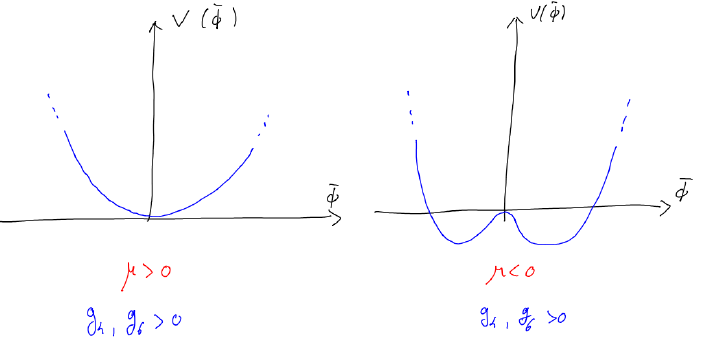
\includegraphics[width=0.9\textwidth]{\main/Images/pot-mu.png}
    \caption{Graph of $V(\bar{\phi})$ (\ref{eqn:V-lattice}) near $\bar{\phi}=0$ for different values of coefficient $\mu$, assuming $g_4, g_6 > 0$.}
    \label{fig:pot-mu}
\end{figure}

So it is reasonable to identify $\mu$ with:
\begin{align*}
    \mu \propto \frac{T-T_c}{T_c} 
\end{align*}

Note that this leads to the same phenomenology given by the mean field approximation. However, as we started from a much more general expression (\ref{eqn:H-lattice}), we can now \textit{go beyond} it! One way is to (perturbatively) consider \textit{deviations} from the saddle point solution, i.e. $\phi_x = \bar{\phi} + \varphi_x$. Then the partition function becomes:
\begin{align*}
    Z_{\mathrm{Lattice}} = e^{-N V(\bar{\phi})} \int_{\mathbb{R}^N} \Big[\prod_x \dd{\varphi_x}\Big] \exp\left(-\frac{1}{2} \sum_{xy} \pdv[2]{\mathcal{H}}{\phi_x}{\phi_y} \Big|_{\bm{\phi} = \bm{\bar{\phi}}} \varphi_x \varphi_y + \dots \right)
\end{align*}  

Note that if we keep only the $\mu$ term (Gaussian model), i.e.:
\begin{align*}
    V(\phi) = \frac{\mu}{2} \phi^2 
\end{align*}
Then the saddle point approximation (with uniform solution) leads to:
\begin{align*}
    0 \overset{!}{=} V'(\bar{\phi}) = \mu \bar{\phi} \Leftrightarrow \bar{\phi} = 0
\end{align*}
So the (mean field) Gaussian model can describe only the paramagnetic phase - as there is no equivalent of the spontaneous magnetization (\ref{eqn:emergent-sol}).

\subsection{The Lattice Gaussian Model}
As an example, let's examine what happens if we keep only the first gradient term and the $\mu$ term in (\ref{eqn:Z-lattice}):
\begin{align} \nonumber
    -\beta H_{G, \mathrm{Lattice}}(\bm{\phi}) &= \frac{1}{2} \sum_{\langle x,y \rangle} (\phi_x - \phi_y)^2 + \frac{\mu}{2} \sum_x \phi_x^2 =\\ \nonumber
    &= \frac{1}{2} \Big[\sum_{\langle x,y \rangle} (\phi_x^2 + \phi_y^2)
    +\mu \sum_x \phi_x^2 \Big]
    - \sum_{\langle x,y \rangle} \phi_x \phi_y =  \\ \nonumber
    &\underset{(a)}{=}  \frac{1}{2}\Big[ 2d \sum_x \phi_x^2 + \mu \sum_x \phi_x^2 \Big]  - \sum_{\langle x,y \rangle} \phi_x \phi_y = \\ \nonumber
    &= \frac{1}{2}\sum_{x} \phi_x^2 (\mu + 2d) - \sum_{\langle x,y \rangle}  \phi_x \phi_y =\\ \nonumber
    &= \frac{1}{2} \sum_{xy} \phi_x (\mu + 2d) \delta_{xy} \phi_y - \sum_{xy} \phi_x \phi_y \delta_{|\bm{r}_x - \bm{r}_y|,1} =\\ \nonumber
    &= \frac{1}{2} \sum_{xy} \phi_x M_{xy} \phi_y \\ \label{eqn:gaussian-mtx}
    M_{xy} &= \hlc{Yellow}{(\mu + 2d)\delta_{x,y} }- \hlc{SkyBlue}{\delta_{|\bm{r}_x-\bm{r}_y|,1}}  
\end{align}
where in (a) we used the same reasoning needed for (\ref{eqn:sum3}, pag. \pageref{eqn:sum3}).

\medskip

To proceed, note that the matrix $M_{xy}$ is just the inverse of the \textit{covariance matrix} of a multidimensional gaussian, meaning that:
\begin{align*}
    \langle \phi_x \phi_y \rangle = M_{xy}^{-1}
\end{align*} 
Moreover, the form of (\ref{eqn:gaussian-mtx}) strongly resembles that of the correlation matrix we computed in the mean field (\ref{eqn:G-mtx}, pag. \pageref{eqn:G-mtx}):
\begin{align*}
    G_{xy}^{-1} = \frac{1}{1-m^2} \delta_{xy} - K_{xy} = \begin{cases}
        \hlc{Yellow}{\frac{1}{1-m^2}} & x=y\\
        \hlc{SkyBlue}{-K} & |\bm{r}_x-\bm{r}_y| = a 
    \end{cases}  
\end{align*}
where the corresponding elements are highlighted with the same color. We already diagonalized $G_{xy}$ in (\ref{eqn:G-eigenvalue}, pag. \pageref{eqn:G-eigenvalue}):
\begin{align}\label{eqn:G-diag}
    G_{xy} = \left(\frac{a}{2\pi} \right)^{d} \int_{\left(-\frac{\pi}{a},+\frac{\pi}{a}  \right)^d} \dd[d]{\bm{p}} e^{i \bm{p} \cdot (\bm{r}_x - \bm{r}_y)} \underbrace{\frac{1}{\displaystyle \hlc{Yellow}{(1-m^2)^{-1}} - \hlc{SkyBlue}{2K \sum_{\mu=1}^d \cos(a p_\mu)}}}_{\tilde{G}(\bm{p})}
\end{align}
And so by comparing (\ref{eqn:gaussian-mtx}) with (\ref{eqn:G-diag}) we find:
\begin{align*}
    \langle \phi_x \phi_y \rangle = M_{xy}^{-1} = \left(\frac{a}{2\pi} \right)^d \int_{\left(-\frac{\pi}{a}, \frac{\pi}{a}\right)} \dd[d]{\bm{p}} e^{i \bm{p}(\bm{r}_x - \bm{r}_y)} \frac{1}{\displaystyle \hlc{Yellow}{\mu + 2d} - \hlc{SkyBlue}{2 \sum_{\mu=1}^d \cos(p_\mu a)}} 
\end{align*}
where we also reintroduced $a \neq 1$. Thus, the eigenvalues $M(\bm{p})$ of $M_{xy}$ are:
\begin{align*}
    M(\bm{p}) = \Big[\frac{1}{\mu + 2d - 2 \sum_{\mu=1}^d \cos(p_\mu a)} \Big]^{-1} = \mu + 2d - 2 \sum_{\mu=1}^d \cos(p_\mu a)
\end{align*}
Then, in the stationary phase approximation, we expand around $\bm{p} = \bm{0}$ (as we did in (\ref{eqn:eigenvalue-expansion})):
\begin{align*}
    M(\bm{p}) = \mu + \norm{p} a^2 + O(\norm{\bm{p}}^4) = a^2 \left(\frac{\mu}{a^2} + \norm{\bm{p}}^2 \right) + O(\norm{\bm{p}}^4)
\end{align*}
Noting that $[\mu^{-1} a^2] = \sf{L}^2$, we define the correlation length $\xi \equiv \sqrt{a^2 \mu^{-1}}$. As $\mu \propto t$, this means:
\begin{align*}
    \xi \equiv \sqrt{a^2 \mu^{-1}} \propto \left(\frac{T-T_c}{T_c} \right)^{-\nu} \qquad \nu = \frac{1}{2} 
\end{align*}
Which is exactly the same result we got in the mean field approximation.

\section{Conclusions}
\begin{enumerate}
    \item The continuum limit of a generic Ising Model (\ref{eqn:continuum-limit}) suggests that the lattice Hamiltonian (\ref{eqn:H-lattice}) with continuous field $\phi$ and only a \textbf{few terms} capture the correct critical behaviour of an \textit{infinite} class of detailed models with \textbf{short-range interactions}.
    \item The number of significant terms depends on the model's \textbf{dimensionality}. In particular:
    \begin{itemize}
        \item When $d > 4 \equiv d_c$ (critical dimension) the critical behaviour is the one captured by the \textbf{mean field approximation}, and the Gaussian model describes the $2$-point correlation.
        \item When $3 < d \leq 4$, we consider an additional term:
        \begin{align} \label{eqn:z2-H}
            \beta \mathcal{H}_{\mathrm{Lattice}}(\bm{\phi}) = \sum_{\langle x,y \rangle} \frac{1}{2} (\phi_x - \phi_y)^2 -\frac{\mu}{2}\sum_x \phi_x^2 + g \sum_x \phi_x^4 
        \end{align}
        This is known as the $\phi^4$-model, and it's the paradigm for describing second order phase transitions in the universality class of systems with $\mathbb{Z}_2$ symmetry.

        \medskip

        (\ref{eqn:z2-H}) can be generalized to other kinds of symmetries. For example, a generic Hamiltonian with $O(n)$ symmetry is given by:
        \begin{align*}
            - \beta H(\{\bm{s}\}) = K \sum_{\langle x,y \rangle} \bm{s_x} \cdot \bm{s_y} + L \sum_{\langle \langle x,y \rangle \rangle} \bm{s_x} \cdot \bm{s_y} + M \sum_{[xyzt]} (\bm{s_x} \cdot \bm{s_y}) (\bm{s_z} \cdot \bm{s_t}) + \dots
        \end{align*}
        In this case, (\ref{eqn:z2-H}) becomes:
        \begin{align*}
            \beta \mathcal{H}_{\mathrm{Lattice}}(\bm{\phi}) = \sum_{\langle x,y \rangle} \frac{1}{2} (\bm{\phi_x} - \bm{\phi_y})^2 - \frac{\mu}{2} \sum_x \norm{\bm{\phi}_x}^2  + g\sum_x \norm{\bm{\phi_x}}^4 
        \end{align*}
    \end{itemize}
\end{enumerate}

\chapter{Dynamics}
Until now, apart from the chapter on irreversibility, we were only interested in equilibrium properties. Now we shift our focus to the \textbf{dynamics} of complex systems. 

\medskip

We will start by introducing Markov Processes, which are the simplest non-trivial models for describing the evolution of a system.
%TODO Complete introduction


\section{Markov Processes}
Consider a \textbf{discrete} set of events $E$, representing the system's states. For example, $m \in E$ could be a particular configuration of spins $\bm{\sigma} = (\sigma_1,\dots,\sigma_N)$ in the IM, and in this case $|E| = 2^N$ with $N$ being the number of spins. 

\medskip

A Markov Process describes a \q{memoryless evolution}, in which the current state of the system at a certain time $t$ is the only information needed to compute the \textbf{transition probabilities} to any other state $m'$ at a future time $t' > t$. 

In other words, if a system is at state $m$ at time $t$, then the probability that it will move to state $m'$ at time $t' > t$ is given by $\mathbb{P}(m',t'|m,t)$, which does not depend on the previously traversed states at times $\hat{t} < t$.

\medskip

This means that the \textit{joint} probability of a \textit{specific} evolution of the system, which at time $t_i$ is in state $m_i$, can be factorized as follows:\marginpar{\vspace{2em}Markov Property}
\begin{align}\label{eqn:Markov-property}
    \mathbb{P}(m_k, t_k; m_{k-1}, t_{k-1}; \dots; m_1, t_1) = \span\\
    = \mathbb{P}(m_k, t_k|m_{k-1}, t_{k-1}) \mathbb{P}(m_{k-1}, t_{k-1}|m_{k-2}, t_{k-2}) \cdots \mathbb{P}(m_2, t_2|m_1, t_1) \mathbb{P}(m_1, t_1)\span \nonumber
\end{align}
where $t_1 < t_2 < \cdots < t_k$ are arbitrary instants.
(\ref{eqn:Markov-property}) is indeed the \textit{defining} property of a Markov Process.  

\medskip

Markov Processes are the simplest kind of stochastic processes that are non-trivial, as they incorporate a \textit{slight} dependence on the past. 

A \textit{trivial} process would be one for which the probability of each state is \textit{completely independent on the previous states}, meaning that $\mathbb{P}(m',t'|m,t) = \mathbb{P}(m',t')$. 

\medskip

Note that, by definition, the \q{transition probability to the present} is given by:
\begin{align*}
    \mathbb{P}(m',t|m,t) = \delta_{m',m}
\end{align*}

\medskip

We will call $\mathbb{P}(m, t| m_0, t_0)$ the \textbf{propagator}. Starting from an initial distribution over the states $\mathbb{P}(m, t_0)$, the probability of each state $m$ being visited at time $t$ is given by:
\begin{align}\label{eqn:propagator-evolution}
    \mathbb{P}(m,t) = \sum_{m_0} \mathbb{P}(\underset{\mathrm{end}}{m,t} |\underset{\mathrm{start}}{m_0,t_0} ) \mathbb{P}(m_0,t_0)
\end{align}
In a sense, $\mathbb{P}(m,t|m_0,t_0)$ \q{propagates} the initial distribution to the evolved one.

\medskip

Clearly, for a Markov Process $\mathbb{P}(m,t|m_0,t_0)$ must be compatible with (\ref{eqn:Markov-property}). Our goal is then to derive a differential equation for the propagator, containing some detail about the specific dynamics of the system.

\subsection{Chapman-Kolmogorov equation}
Let's start by considering three instants $t_0 < t' < t$. The conditional probability for a system to visit state $m$ at $t$ and state $m'$ at $t'$, given it started in $m_0$ at $t_0$ is given by:
\begin{align*}
    \mathbb{P}(m,t;m',t'|m_0,t_0)
\end{align*}
Due to the Markov Property (\ref{eqn:Markov-property}) this can be rewritten as:
\begin{align*}
    \mathbb{P}(m,t;m',t'|m_0,t_0) = \mathbb{P}(m,t|m',t') \mathbb{P}(m',t'|m_0,t_0)
\end{align*}
Marginalizing over $m'$:
\begin{align}\label{eqn:chapman-kolmogorov}
    \mathbb{P}(m,t|m_0,t_0) = \sum_{m'} \mathbb{P}(m,t;m',t'|m_0,t_0) = \sum_{m'} \mathbb{P}(m,t|m',t') \mathbb{P}(m',t'|m_0,t_0) \quad \forall t' \in (t_0,t)
\end{align}
This is the so-called Chapman-Kolmogorov equation. 

\section{Master Equation}

To get a differential equation for the propagator, we choose $t' = t - \Delta t$, with $\Delta t \approx 0$. Substituting in (\ref{eqn:chapman-kolmogorov}) and separating the terms with $m' \neq m$ from the one with $m' = m$ we get:
\begin{align}\nonumber
    \mathbb{P}(m,t|m_0,t_0) &= \sum_{m' \neq m} \Big[\mathbb{P}(m,t|m',t-\Delta t) \mathbb{P}(m', t-\Delta t|m_0,t_0)\Big] +\\
    &\quad\> +\hlc{Yellow}{ \mathbb{P}(m,t|m,t-\Delta t)}\mathbb{P}(m,t-\Delta t|m_0,t_0) \label{eqn:ck-split}
\end{align}
As the system is always in some state, the transition probabilities to all possible states $m'$ must sum to $1$:
\begin{align*}
    \sum_{m'} \mathbb{P}(m',t|m,t-\Delta t) \overset{!}{=}  1
\end{align*}
Splitting the sum over $m \neq m'$ and $m = m'$ leads to:
\begin{align*}
    \Big[\sum_{m' \neq m} \mathbb{P}(m',t|m,t-\Delta t)\Big] + \mathbb{P}(m,t|m,t-\Delta t) = 1
\end{align*}
And rearranging:
\begin{align*}
    \mathbb{P}(m,t|m,t-\Delta t) = \hlc{Yellow}{1- \sum_{m' \neq m} \mathbb{P}(m',t|m,t-\Delta t)}
\end{align*}
Which can then be substituted in (\ref{eqn:ck-split}):
\begin{align}\label{eqn:ck-2}
    \mathbb{P}(m,t|m_0,t_0) - \mathbb{P}(m, t-\Delta t|m_0,t_0) = \span\\ \nonumber
    = \sum_{m' \neq m} \Big[\mathbb{P}(m,t|m',t-\Delta t) \mathbb{P}(m',t- \Delta t|m_0,t_0) - \mathbb{P}(m',t|m,t-\Delta t) \mathbb{P}(m,t-\Delta t|m_0,t_0)\Big] \span
\end{align}

We now assume that the \textit{transition probability per unit time $\Delta t$} has a finite limit for $\Delta t \to 0$:
\begin{align*}
    \lim_{\Delta t \to 0} \frac{1}{\Delta t} \mathbb{P}(m',t|m,t-\Delta t) \equiv W_t(\underset{\mathrm{end}}{m'} |\underset{\mathrm{start}}{m} )
\end{align*}   
where $W_t(m'|m)$ is the \textbf{transition rate} from $m$ to $m'$. Then, for a small $\Delta t \approx 0$, the probability of the system jumping from state $m$ to state $m'$ in the time interval $(t,t+\Delta t)$ is given by $W_t(m'|m) \Delta t$.  

\medskip

Then, taking the limit $\Delta t \to 0$ of both sides of (\ref{eqn:ck-2}) leads to:
\begin{align*}
    \lim_{\Delta t \to 0} \mathbb{P}(m,t|m_0,t_0) - \mathbb{P}(m,t-\Delta t|m_0,t_0) = \partial_t \mathbb{P}(m,t|m_0,t_0) \Delta t = \span \\
    =\sum_{m'} [\hlc{Yellow}{W_t(m|m') }\Delta t \mathbb{P}(m',t|m_0,t_0) - \hlc{SkyBlue}{W_t(m'|m)} \Delta t \mathbb{P}(m,t|m_0,t_0)]  \span
\end{align*}
Here the sum can be taken over all $m'$, as the $m=m'$ term automatically cancels out. Note that the yellow term describes jumps \textbf{to}  $m$ (an \q{inward} flow of probability) and the blue term jumps \textbf{from} $m$ to another state (an \q{outward} flow of probability).

\begin{figure}[H]
    \centering
    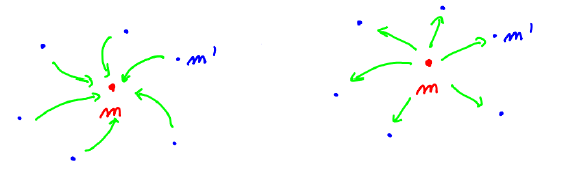
\includegraphics[width=0.8\textwidth]{\main/Images/probability-flows.png}
    \caption{$W_t(m|m')$ measures the \textit{probability flow} \textbf{entering} $m$ (left), while $W_t(m'|m)$ is the one \textbf{exiting} $m$ (right).}
    \label{fig:probability-flows}
\end{figure}

Then, dividing everything by $\Delta t$:\marginpar{\vspace{2em}Master Equation}
\begin{align}\label{eqn:MasterEquation}
    \partial_t \mathbb{P}(m,t|m_0,t_0) = \sum_{m'} \Big[ W_t(m|m') \mathbb{P}(m',t|m_0,t_0) - W_t(m'|m) \mathbb{P}(m,t|m_0,t_0)\Big]
\end{align}
which is known as the \textbf{Master Equation}. 

If we multiply both sides by $\mathbb{P}(m_0,t_0)$ and sum over $m_0$, using (\ref{eqn:propagator-evolution}) leads to:
\begin{align}\label{eqn:master-evolution}
    \partial_t \mathbb{P}(m,t) = \sum_{m'} \Big[W_t(m|m') \mathbb{P}(m',t) - W_t(m'|m) \mathbb{P}(m,t) \Big]
\end{align}

If transition rates $W_t(m|m')$ do not depend on $t$, the Markov Process is said to be \textbf{homogeneous}. In this case (\ref{eqn:master-evolution}) reduces to:\marginpar{\vspace{2em}Time evolution of the pdf}
\begin{align}\label{eqn:pdf-evolution}
    \partial_t \mathbb{P}(m,t) = \sum_{m'} \Big[W(m|m') \mathbb{P}(m',t) - W(m'|m)\mathbb{P}(m,t)\Big]
\end{align}
In a sense this is analogous to the Fokker-Planck equation for Brownian Motion, with the right hand side representing a \textit{probability current}. 

By equating $\partial_t \mathbb{P}(m,t) = 0$ we can find a \textbf{stationary state} $\mathbb{P}_0(m)$, which is the solution (if it exists) of:\marginpar{\vspace{2em}Stationary states}
\begin{align}\label{eqn:stationary-equation}
    \sum_{m'} \Big[W(m|m') \mathbb{P}_0(m') - W(m'|m) \mathbb{P}_0(m)\Big]  = 0
\end{align} 

$\mathbb{P}_0(m)$ is a stationary \textbf{equilibrium state} if each single term in the sum (\ref{eqn:stationary-equation}) is zero:\marginpar{\vspace{1em}Detailed Balance and Equilibrium State}
\begin{align}\label{eqn:detailed-balance}
    \hlc{SkyBlue}{W(m|m') \mathbb{P}_{\mathrm{eq}}(m')} = \hlc{ForestGreen}{W(m'|m) \mathbb{P}_{\mathrm{eq}}(m)} 
\end{align}
This is the so-called \textbf{detailed balance} condition. An equilibrium state is such that the \textit{probability flows} between each pair of states are perfectly balanced, meaning that there is no net \q{motion of probability} anywhere. 

\begin{figure}[H]
    \centering
    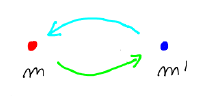
\includegraphics[width=0.4\textwidth]{\main/Images/detailed-balance.png}
    \caption{If detailed balance (\ref{eqn:detailed-balance}) holds, the probability flow $W(m|m')\mathbb{P}_{\mathrm{eq}}(m)$ from $m'$ to $m$ is exactly equal to the one $W(m'|m)\mathbb{P}_{\mathrm{eq}}(m)$ from $m$ to $m'$.}
    \label{fig:detailed-balance}
\end{figure}

As probabilities are always positive, we can write $\mathbb{P}_{\mathrm{eq}}$ as a Boltzmann probability for a certain energy function $\mathcal{E}(m)$:
\begin{align*}
    \mathbb{P}_{\mathrm{eq}}(m) = \frac{1}{Z} e^{-\beta \mathcal{E}(m)} \qquad Z \equiv \sum_{m} e^{-\beta \mathcal{E}(m)}
\end{align*}
Then (\ref{eqn:detailed-balance}) implies:\marginpar{\vspace{2em}Freedom in the transition rates choice}
\begin{align}\label{eqn:transition-energy-rates}
    \frac{W(m|m')}{W(m'|m)} = e^{-\beta [\mathcal{E}(m) - \mathcal{E}(m')]} 
\end{align}
There are \textit{infinite} possible choices for the transition rates $W(i,j)$ that satisfy (\ref{eqn:transition-energy-rates}). In fact, if $W(m|m')$ is such that (\ref{eqn:transition-energy-rates}) holds, then we can construct a new $W'(m|m')$ as follows:
\begin{align*}
    W'(m|m') = W(m|m') C(m,m')
\end{align*}
For some function $C(m,m')$ of the states. If we choose $C(m,m') = C(m',m)$ (i.e. it is a \textit{symmetric} function)
then $W'(m|m')$ satisfies (\ref{eqn:transition-energy-rates}) too.

This means that if we arbitrarily choose some form for the transition rates, as long as they do satisfy (\ref{eqn:detailed-balance}), we are sure that the stationary state \textbf{corresponds} to the system's equilibrium.

\medskip

However, it is not clear if the system dynamics will \textit{lead} to a stationary state for any initial condition. This is really not a trivial matter - nonetheless fortunately, if (\ref{eqn:detailed-balance}) holds, it can be shown (see sec. \ref{sec:proof-db}) that the equilibrium state will be eventually reached. 

\medskip

If we sum over $m$ both sides of the Master Equation (\ref{eqn:MasterEquation}), the right hand side vanishes, leading to:
\begin{align*}
    \pdv{t} \sum_m \mathbb{P}(m,t) = 0 \Leftrightarrow \sum_{m} \mathbb{P}(m,t) = \text{Independent of $t$}
\end{align*}
This means that the total probability never changes, i.e. it is conserved:\marginpar{\vspace{1em}Conservation of Probability}
\begin{align}\label{eqn:conservation-of-probability}
    \sum_{m} \mathbb{P}(m,t) = \sum_{m} \mathbb{P}(m,0) = 1
\end{align}

Using the Master Equation we can also compute the evolution of the \textit{average} of a generic function $f$ of the state:\marginpar{\vspace{1em}Evolution of averages}
\begin{align*}
    \langle f \rangle_t \equiv \sum_m \mathbb{P}(m,t) f(m)
\end{align*}
Differentiating with respect to $t$:
\begin{align} \nonumber
    \partial_t \langle f \rangle_t &= \sum_m \partial_t \mathbb{P}(m,t) f(m) \underset{(\ref{eqn:pdf-evolution})}{=}  \sum_{m,m'} f(m) \Big[ W(m|m')\mathbb{P}(m',t) - W(m'|m)\mathbb{P}(m,t)\Big] =\\ \nonumber
    &= \sum_{m,m'} f(\textcolor{Red}{m'}) W(\textcolor{Red}{m'}|\textcolor{Blue}{m}) \mathbb{P}(\textcolor{Red}{m'},t) - \sum_{m, m'} f(m) W(m'|m)\mathbb{P}(m,t) = \\ 
    \shortintertext{Exchanging $m \leftrightarrow m'$ in the first sum (which is allowed since we are summing over both $m$ and $m'$, and so it just amounts to a \textit{reordering} of addends) allows us to collect a $\mathbb{P}(m,t)$ factor:} \nonumber
    &= \sum_{m,m'} f(\textcolor{Blue}{m}) W(\textcolor{Blue}{m}|\textcolor{Red}{m'}) \mathbb{P}(\textcolor{Blue}{m},t) - \sum_{m,m'} f(m) W(m'|m) \mathbb{P}(m,t) =\\ \label{eqn:evolution-of-averages}
    &= \sum_m \mathbb{P}(m,t) \sum_{m'} \Big[f(m') W(m'|m) - f(m) W(m'|m) \Big]
\end{align}
In this way, the last expression can be interpreted as the \textit{average} of the quantity in the square brackets. 

\medskip

The same result can be obtained by using a more synthetic notation. First, we rewrite (\ref{eqn:pdf-evolution}) as a matrix product. Let $\bm{P}(t)$ be the vector of probabilities $(\mathbb{P}(m,t)\colon m \in E)$. Our target is an expression as the following:\marginpar{\vspace{1em}Evolution of a pdf: matrix form}
\begin{align}\label{eqn:pdf-evolution-matrixform}
    \dot{\bm{P}}(t) = \mathrm{T} \bm{P}(t)
\end{align}
for some matrix $\mathrm{T}$. To find it, we need to convert (\ref{eqn:pdf-evolution}) to the form:
\begin{align*}
    \partial_t \mathbb{P}(m,t) = \sum_{m'} T_{m,m'} \mathbb{P}(m',t)
\end{align*}
Note that the first term in (\ref{eqn:pdf-evolution}) is already in the correct form:
\begin{align}\label{eqn:pdf-evolution2}
    \partial_t \mathbb{P}(m,t) = \sum_{m'} \Big[W(m|m') \mathbb{P}(m',t) - W(m'|m)\mathbb{P}(m,t)\Big]
\end{align}
To \q{adapt} also the second one, we first rename $m'$ to $m''$, and then insert a sum with a Kronecker delta to \q{convert} the $m$ to $m'$:
\begin{align*}
    \sum_{\textcolor{Red}{m'}} W(\textcolor{Red}{m'}|m) \mathbb{P}(m,t) = \sum_{\textcolor{Red}{m''}} W(\textcolor{Red}{m''}|m) \mathbb{P}(m,t) = \textcolor{Blue}{\sum_{m}} \sum_{m''} W(m''|\textcolor{Blue}{m'}) \mathbb{P}(\textcolor{Blue}{m'},t) \textcolor{Blue}{\delta_{m,m'}}
\end{align*}
Substituting in (\ref{eqn:pdf-evolution2}) and collecting a $\mathbb{P}(m',t)$:
\begin{align}\label{eqn:evo-matrix}
    \partial_t \mathbb{P}(m,t) = \sum_{m'} \underbrace{\Big[W(m|m') - \delta_{m,m'} \sum_{m''} W(m''|m') \Big]}_{T(m,m')}  \mathbb{P}(m',t)
\end{align}
And so we find:
\begin{align} \label{eqn:T-matrix}
    T(m,m') \equiv W(m|m') - \delta_{m,m'} \sum_{m''} W(m''|m')
\end{align}

Let's define the (symmetric) scalar product of two functions $f, g\colon E \to \mathbb{R}$ as follows:
\begin{align*}
    \langle f|g \rangle = \sum_{m} f(m) g(m) = \langle g|f \rangle
\end{align*}
Then, the average of $f$ at time $t$ can be written as:
\begin{align*}
    \langle f \rangle_t = \langle f | \bm{P}(t) \rangle
\end{align*}
And differentiating with respect to $t$:
\begin{align} \label{eqn:average-evolution-matrix}
    \partial_t \langle f \rangle_t = \langle f|\partial_t \bm{P}(t) \rangle \underset{(\ref{eqn:pdf-evolution-matrixform})}{=}  \langle f | \mathrm{T} \bm{P}(t) \rangle = \langle \mathrm{T}^T f| \bm{P}(t) \rangle = \langle \mathrm{T}^T f \rangle
\end{align}
However $\mathrm{T}$ (\ref{eqn:T-matrix}) is symmetric:
\begin{align}\label{eqn:T-symmetry}
    \mathrm{T}^T(m,m') = \mathrm{T}(m',m)
\end{align}
And so:
\begin{align*}
    \langle \mathrm{T}^T f \rangle = \sum_{m'} \mathrm{T}^T(m,m') f(m')\> \underset{\mathclap{(\ref{eqn:T-symmetry})}}{=}\> \sum_{m'} f(m') \mathrm{T}(m',m) \>\underset{\mathclap{(\ref{eqn:T-matrix})}}{=} \> \sum_{m'} [f(m') W(m'|m) - f(m) W(m'|m)]
\end{align*}
which is exactly the result we found in (\ref{eqn:evolution-of-averages}).

\begin{example}[Homogeneous Poisson Process]
    Consider a store, and denote with $\mathbb{P}(n,t)$ the probability that $n \in \mathbb{N}$ customers have visited it after a time $t$. 
    
    If clients arrive with a fixed rate $\lambda$ (arrivals per unit time), then the transition rate from a state with $n-1$ clients to one with $n$ clients is exactly $\lambda$:
    \begin{align*}
        W(n|n-1) = \lambda
    \end{align*}
    Supposing that no more than one customer can enter the shop at the same time, all the other rates are null:
    \begin{align*}
        W(n|n') = 0 \quad \forall n' \neq n-1
    \end{align*}
    Then (\ref{eqn:pdf-evolution}) becomes:
    \begin{align*}
        \partial_t \mathbb{P}(n,t) &= \lambda(\mathbb{P}(n-1,t) - \mathbb{P}(n,t)) = \sum_{n'} T(n,n') \mathbb{P}(n',t)\\
        T(n,n') &\underset{(\ref{eqn:T-matrix})}{=} (\delta_{n',n-1} - \delta_{n,n'}) \lambda \cdot \bb{1}_{n' \geq 0} \qquad \bb{1}_{n' \geq 0} = \begin{cases}
            1 & n' \geq 0\\
            0 & \text{otherwise}
        \end{cases}
    \end{align*}
    The average number of clients evolve as:
    \begin{align*}
        \partial_t \langle n \rangle_t &= \sum_{n=0}^{+\infty} \dot{\mathbb{P}}(n,t) n = \lambda \sum_{n=0}^{+\infty} \left[\mathbb{P}(n-1,t) - \mathbb{P}(n,t)\right] n
        \intertext{Note that the $n=0$ term vanishes, and so the first nonzero term is the one with $n=1$. Shifting the sum leads to:}
        &= \lambda \left[\sum_{n=0}^{+\infty} \mathbb{P}(n,t)(n+1) - \sum_{n=0}^{+\infty} \mathbb{P}(n,t)n\right] = \\
        &= \lambda \underbrace{\sum_{n=0}^{+\infty} \mathbb{P}(n,t)}_{1 \> (\ref{eqn:conservation-of-probability})}  = \lambda
    \end{align*}
    Integrating over $t$ we get:
    \begin{align}\label{eqn:n-average}
        \langle n \rangle_t = \langle n \rangle_0 + \lambda t
    \end{align}
    As expected, the number of clients that have visited the shop increases linearly, with a \textit{speed} equal to the rate $\lambda$.
    
    \medskip

    We can then compute the \textbf{variance} $\operatorname{Var}(n)_t$. To do so, we use the moment-generating properties of the \textit{probability generating function}:
    \begin{align}\label{eqn:G-genfunc}
        G(z,t) = \langle g \rangle_t = \sum_{n=0}^{+\infty} z^n \mathbb{P}(n,t) \qquad g(n) \equiv z^n
    \end{align}    
    As $g(n)$ is a function of the state, the evolution of its average is given by (\ref{eqn:average-evolution-matrix}):
    \begin{align*}
        \partial_t G(z,t) = \langle \mathrm{T}^T g \rangle_t
    \end{align*}
    which evaluates to:
    \begin{align*}
        (\mathrm{T}^T g)(n) &= \sum_{n'} T(n',n) g(n') = \lambda \sum_{n'} (\delta_{n, n'-1} - \delta(n,n') \bb{1}_{n \geq 0}) z^{n'} = \\
        &= \lambda z^n (z-1) = \lambda (z-1) g(n)
    \end{align*}
    And so:
    \begin{align}\label{eqn:G-avg-evo}
        \partial_t G(z,t) = \lambda (z-1) G(z,t)
    \end{align}
    Notice that if $z=1$:
    \begin{align*}
        G(1,t) = \sum_{n \geq 0} \mathbb{P}(n,t) = 1
    \end{align*}
    And (\ref{eqn:G-avg-evo}) with $z=1$ is just the probability conservation (\ref{eqn:conservation-of-probability}):
    \begin{align*}
        \partial_t G(1,t) = 0
    \end{align*}

    We can then integrate (\ref{eqn:G-avg-evo}) with initial condition $\mathbb{P}(n,0) = \delta_{n,0}$:
    \begin{align*}
        \begin{cases}
            \partial_t G(z,t) = \lambda (z-1) G(z,t)\\
            G(z,0) = \sum_{n} z^n \mathbb{P}(n,0) = 1
        \end{cases} \span \\ \Rightarrow G(z,t) = e^{\lambda (z-1)t} = e^{- \lambda t} \sum_{n=0}^{+\infty} z^n \frac{(\lambda t)^n}{n!} \underset{(\ref{eqn:G-genfunc})}{\Rightarrow}  \mathbb{P}(n,t) = e^{-\lambda t} \frac{(\lambda t)^n}{n!} \span
    \end{align*}
    And so $\mathbb{P}(n,t)$ is a Poisson distribution with rate $\lambda$. 
    
    Finally, recalling the generating properties of (\ref{eqn:G-genfunc}) we can compute the average of $n$, finding again (\ref{eqn:n-average}) with $\langle n \rangle_0 = 0$:
    \begin{align*}
        \langle n \rangle_t = z \pdv{z} G(z,t) \Big|_{z=1} = \lambda t
    \end{align*}
    On the other hand, the fluctuation of $n$ is given by:
    \begin{align*}
        \sigma_t^2 &\equiv \langle n^2 \rangle_t - \langle n \rangle^2_t = \left(z \pdv{z}\right)^2 G(z,t)\Big|_{z=1} - (\lambda t)^2 = \\
        &= z \partial_z [\lambda t z G(z,t)]\Big|_{z=1} - (\lambda t)^2 = \lambda t \Rightarrow \sigma_t = \sqrt{\lambda t}
    \end{align*}
\end{example}

\begin{exo}[Radioactive Decay]
    Solve the case of the decay process of radioactive nuclei. Let $\lambda$ be the decay rate, meaning that the transition rates are:
    \begin{align*}
        W(n-1|n) = \lambda \qquad W(n'|n) = 0 \quad \forall n' \neq n-1
    \end{align*}
    Find the law of decay (i.e. the distribution of $n(t)$) given the initial condition $\mathbb{P}(n,0) \equiv \delta_{N,n}$.
\end{exo}

%\subsection{Limiting distribution and equilibrium}
%Added section 7-13


\end{document}
